\documentclass[conference]{IEEEtran}
\IEEEoverridecommandlockouts
% The preceding line is only needed to identify funding in the first footnote. If that is unneeded, please comment it out.
\usepackage{cite}
\usepackage{amsmath,amssymb,amsfonts}
\usepackage{algorithmic}
\usepackage{graphicx}
\usepackage{textcomp}
\usepackage{xcolor}
\def\BibTeX{{\rm B\kern-.05em{\sc i\kern-.025em b}\kern-.08em
    T\kern-.1667em\lower.7ex\hbox{E}\kern-.125emX}}
\begin{document}

\title{Projektarbeit: Unmanned Surface Vehicle\\
}

\author{\IEEEauthorblockN{Josephine Brauer}
\\
\and
\IEEEauthorblockN{Kilian Schweppe}
\\
}

\maketitle

\begin{abstract}
In dieser Projektarbeit wurde ein im Rahmen einer Bachelorarbeit entwickeltes Oberflächenfahrzeug für Wasserexploration in Rettungsszenarien durch Software ergänzt, die es ermöglicht, autonom ein Gewässer abzufahren und dabei die Wassertiefe zu erfassen.\\
Die notwendigen Funktionalitäten wurden in Python unter Nutzung von ROS und des von ROS bereitgestellten Navigation Stacks implementiert. Um die Funktionsweise testen zu können, wurde außerdem eine Simulation des Bootes auf Basis eines bestehenden Simulators erstellt.\\
\end{abstract}

\section{Einleitung}
Mit dem Anstieg der Anzahl der Naturkatastrophen und ihren verursachten Kosten\cite{b1}, nimmt auch die Notwendigkeit zu,  Möglichkeiten für die Verhinderung und Bewältigung von Katastrophen zu finden. Auch die Robotik bietet immer wieder Lösungen, die im Katastrophenschutz eingesetzt werden. Dabei haben Unbemannte Fahrzeuge insbesondere zur Erfassung von Daten ein großes Potenzial \cite{b2}.\\
Sie können Einsatzkräfte in unzugänglichen oder gefährlichen Umgebungen ersetzen \cite{b3}, welche damit sowohl geschützt, als auch anderen Aufgaben zugeteilt werden können.  Durch die potenziell geringe Größe und Lautstärke der Fahrzeuge können auch Gebiete erfasst werden, die sonst entweder nicht zugänglich wären, oder unter größeren Eingriffen in die Natur leiden könnten, wie zum Beispiel Naturschutzgebiete.\\
Besonders für lang andauernde Aufgaben und in Regionen, in denen man damit rechnen muss, nicht immer mit dem Fahrzeug kommunizieren zu können, kann es sinnvoll sein, diese Fahrzeuge nicht nur unbemannt, sondern auch autonom zu gestalten, da das Fahrzeug so nicht durchgehend angesteuert werden muss.\\
In Hinsicht auf Katastrophen spielt der Schutz vor Hochwasser in Schleswig-Holstein eine besondere Rolle, da etwa ein Viertel der Landesfläche und mehr als 350.000 Menschen durch Sturmfluten gefährdet sind \cite{b4}. Hier könnten Unbemannte Wasserfahrzeuge zum Beispiel durch frühzeitiges Erkennen von Deichbrüchen helfen. Die denkbaren Anwendungsfelder sind allerdings nicht nur auf den Schutz vor unseren Gewässern begrenzt, vielmehr könnten sie auch den Schutz unserer Gewässer abdecken, etwa durch Identifikation von Verschmutzungen und ihrer Quellen.\\
Für den Einsatz im und auf dem Wasser sind unter anderem Unbemannte Unterwasserfahrzeuge (UUVs) und Unbemannte Oberflächenfahrzeuge (USVs) möglich \cite{b2}. USVs haben dabei den Vorteil, mehr Sensoren über eine längere Zeitdauer tragen zu können und damit mehr verschiedene Messungen gleichzeitig über einen längeren Zeitraum durchführen zu können, wobei sowohl Messungen an der Oberfläche als auch im Wasser möglich sind \cite{b5}. Trotzdem wird ihnen bis jetzt in der Literatur weniger Beachtung gewidmet, als den Unbemannten Unterwasser Fahrzeugen \cite{b2}.\\
Aus den genannten Gründen erscheint uns die Entwicklung autonomer USVs, die für vielfältige Szenarien ausgerüstet sind, sinnvoll. In dieser Arbeit sollen dafür erste notwendige Schritte erfolgen, indem ein im Rahmen einer Bachelorarbeit entwickeltes Oberflächenfahrzeug für Wasserexploration in Rettungsszenarien durch Software ergänzt wird, die das autonome Befahren eines Gewässers ermöglicht. Des Weiteren wollen wir ein Anwendungsszenario, das Erfassen der Wassertiefe implementieren und testen. Um die Funktionsweise des Bootes testen zu können, ohne Gefahr zu laufen, das Boot auf dem Wasser zu verlieren, und zukünftigen Gruppen die Arbeit mit dem Boot zu erleichtern, soll außerdem eine Simulation des Bootes auf Basis eines bestehenden Simulators erstellt werden.

\section{Methoden}
Da auf dem USV bereits ROS installiert und teilweise genutzt wird, liegt es nahe vom von ROS bereitgestellten Navigation Stack \footnote{https://github.com/ros-planning/navigation} Gebrauch zu machen. Dieser bietet viele nützliche Funktionalitäten -unter anderem werden mehrere globale und lokale Planer bereitgestellt- für die autonome Navigation von mobilen Robotern [TODO]. Er wird in einer Vielzahl von Projekten verwendet [TODO] und es gibt mehrere Tutorials zur Benutzung [TODO], weshalb angenommen werden kann, dass die Verwendung des Navigation Stacks die Verständlichkeit des Projekts auch für Außenstehende verbessert.\\
Auf Basis unserer Zielstellung haben wir mehrere Arbeitspakete identifiziert, auf deren Durchführung im Folgenden eingegangen werden soll:
\begin{enumerate}
	\item Auswahl des Simulators
	\item Einarbeitung Simulator
	\item Simulation der Sensoren des Bootes
	\item Simulation der Ausgaben des Bootes
	\item Implementierung der Schnittstellen zum Navigation Stack
	\item Navigation zu Wegpunkten
	\item Erstellung von Wegpunkten auf Basis der Karte
	\item Erfassung der Wassertiefe und Eintragung in Karte
	\item Schnittstellen zum Navigation Stack, Navigation zu Wegpunkten, Erstellung von Wegpunkten auf Basis der Karte und Erfassung der Wassertiefe auf das Boot übernehmen und -wenn notwendig- anpassen
\end{enumerate}
\subsection{Auswahl des Simulators}
Wir haben uns entschieden, das USV im \textit{Unmanned Surface Vehicle Simulator with Realistic Environmental Disturbances} \footnote{https://github.com/disaster-robotics-proalertas/usv\_sim\_lsa} zu simulieren.\\
Der Master-Branch des Simulators benutzt ROS Kinetic. Da auf dem USV aber momentan ROS Melodic läuft und darüber hinaus Kinetic nach April 2021 nicht mehr von ROS unterstützt wird \cite{b10}, hielten wir es für sinnvoll, zu versuchen, den Simulator auf ROS Melodic laufen zu lassen. Trotz des dafür vorhandenen Branches \footnote{https://github.com/disaster-robotics-proalertas/usv\_sim\_lsa/tree/master-melodic} mussten wir dieses Vorhaben letztendlich aus Zeitgründen und aufgrund von für uns nicht lokalisierbaren Problemen abbrechen und mit Kinetic weiterarbeiten.
\subsection{Simulation der Sensoren des Bootes}
Auf dem Boot sind ein GPS-Gerät, ein Kompass, 2 Ultraschallsensoren, eine 360°-Kamera und ein Temperatursensor zur Erfassung von Daten, 2 Motoren für die Fortbewegung und eine 4G/WIFI-Anbindung zur Kommunikation installiert \ref{boot}.\\
\begin{figure}
	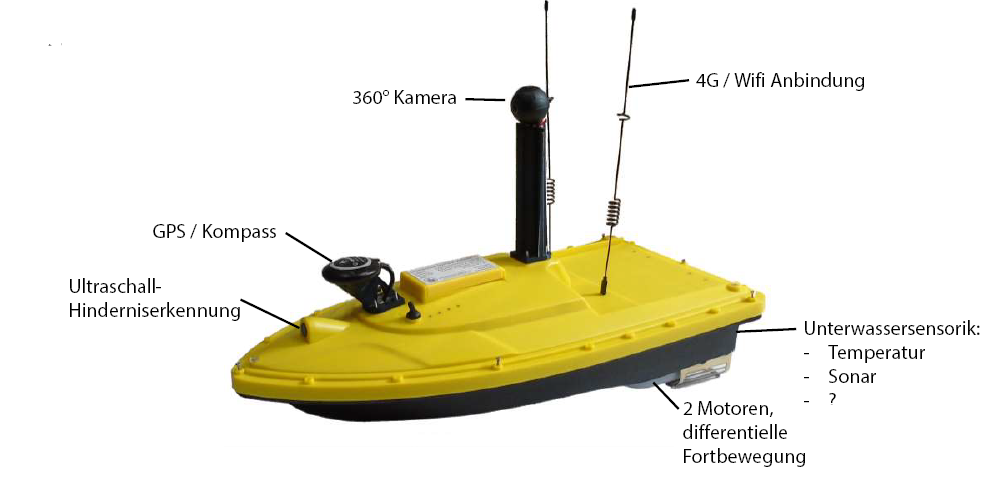
\includegraphics[width=\linewidth]{boot.png}
	\caption{Sensoren des Bootes}
	\label{boot}
\end{figure}
Detaillierte Informationen zu allen Sensoren und Aktuatoren des Bootes und den erwarteten Ein- und Ausgabewerten lassen sich im zugehörigen GitHub-Projekt finden \footnote{https://github.com/NRottmann/UzL\_USV/}.
Für die Implementierung unseres Szenarios in der Simulation benötigten wir die GPS-, Kompass- und Ultraschalldaten und die Motoren. Deshalb haben wir ein GPS-Modul und zwei Ultraschall-Sensoren zum Differentialboot-Modell des Simulators hinzugefügt. Außerdem haben wir das Modell durch eine IMU zur Simulierung der Orientierung ergänzt. Dazu haben wir die GazeboRosGps, GazeboRosImu und GazeboRosSonar Plugins aus dem Paket \textit{hector\_gazebo\_plugins}  \footnote{https://github.com/tu-darmstadt-ros-pkg/hector\_gazebo} verwendet.(TODO: Code)\\
\begin{figure}
	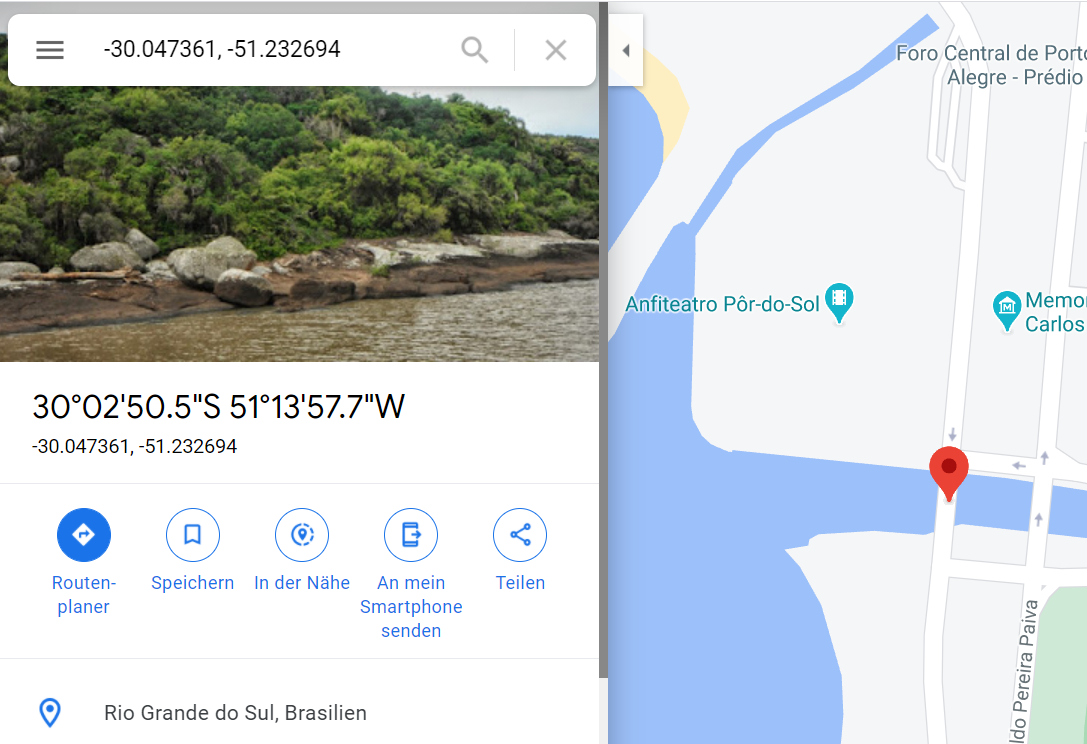
\includegraphics[width=\linewidth]{reference.png}
	\caption{Referenzkoordinaten}
	\label{reference}
\end{figure}\\
Da wir für unser Szenario weitestgehend das \textit{diffboat scenario 1} übernommen haben (das einen Ausschnitt von Porto Alegre, Brasilien, nahe der Mündung des Dilúvio zeigt [1]), haben wir die GPS-Koordinaten eines markanten Punktes im Szenario bestimmt und als Referenzkoordinaten für die Simulierung der GPS-Daten gewählt (\ref{reference}).

\subsection{Simulation der Ausgaben des Bootes}
Nachdem wir die notwendigen Daten simuliert haben, die auch das echte Boot sammelt, wollten wir die Daten auch in derselben Form ausgeben, wie es das USV bereits tut. Dafür haben wir die notwendigen Topics und deren Inhalt bestimmt:
\begin{itemize}
	\item \textit{range\_front}: Daten des vorderen Sonars
	\item \textit{range\_depth}: Daten des unteren Sonars
	\item \textit{velocity}: Geschwindigkeit des Bootes in Bewegungsrichtung
	\item \textit{heading}: unterteilt sich in \textit{gps\_heading}: die Bewegunsrichtung des Bootes und \textit{mag\_heading}: die Orientierung des Bootes
	\item \textit{gps}: GPS-Koordinaten des Bootes
\end{itemize}
\textit{range\_front}, \textit{range\_depth} und \textit{gps} konnten dabei als Parameter im jeweiligen XML-Element gegeben werden (TODO: s. Code). Für das Publishen von \textit{velocity} und \textit{heading} haben wir die Simulationsumgebung durch Skripte ergänzt:\\
Die Geschwindigkeit des Bootes in Bewegungsrichtung, \textit{velocity}, berechnen wir in \textit{TODO} über die Formel:
\begin{equation}
v = \sqrt{x^2+y^2}
\end{equation}
. Dabei ist x die Geschwindigkeit in x-Richtung und y die Geschwindigkeit in y-Richtung. Beide Werte lesen wir aus dem Topic \textit{gps/velocity} aus, welches vom simulierten GPS-Modul gepublisht wird.\\
Für \textit{heading} bestimmen wir die beiden Komponenten \textit{gps\_heading} und \textit{mag\_heading} einzeln:\\
Über 
\begin{equation}
	atan2(x,y) 	
\end{equation}
(wobei wieder x die Geschwindigkeit in x-Richtung und y die Geschwindigkeit in y-Richtung ist) bestimmen wir das \textit{gps\_heading}, also die Bewegungsrichtung nach GPS. \\
Aus der Komponente \textit{orientation} der simulierten IMU kann durch Umwandlung der ausgegebenen Quaternion in Euler-Winkel das \textit{mag\_heading} bestimmt werden.\\
Beide Winkelangaben haben wir noch so angepasst, dass statt bei einer Orientierung Richtung Osten, bei einer Orientierung Richtung Norden 0° vorliegen. Beide Werte werden danach auf das Topic \textit{heading} gepublisht.\\
Auf das Publishen der Topics \textit{mag}, \textit{temperature}, und \textit{safety} haben wir vorerst verzichtet, da diese für unseren Anwendungsfall nicht notwendig waren.

\subsection{Implementierung der Schnittstellen zum Navigation Stack}
Wie in Figure \ref{nav} zu sehen, hat der Roboter die Möglichkeit, Werte auf die Topics \textit{tf}, \textit{odom}, \textit{map}, und \textit{move\_base\_simple/goal}, sowie Sensor Topics des Formates LaserScan oder PointCloud zu publishen und auf das Topic \textit{cmd\_vel} zu subscriben, um mit dem Navigation Stack zu interagieren.\\
Deshalb ist es notwendig, diese Schnittstellen auf dem Boot zu implementieren. Da wir in der Simulation dieselben Ausgabeschnittstellen erzeugt haben, wie wir sie auf dem echten Boot vorliegen haben werden, genügte eine Implementierung der Schnittstellen zum Navigation Stack sowohl für die Simulation als auch für das echte Boot.
\begin{figure}
	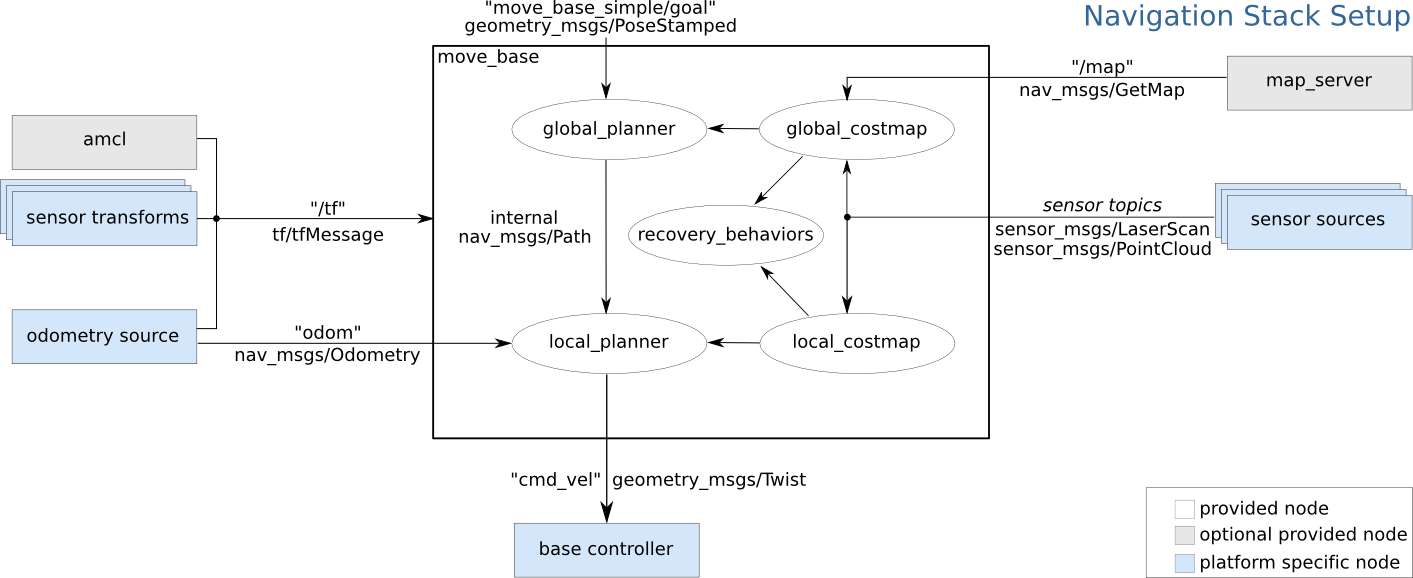
\includegraphics[width=\linewidth]{overview_tf.png}
	\caption{Robot Setup Navigation Stack (Quelle: http://wiki.ros.org/navigation/Tutorials/RobotSetup (Stand: 2018-07-19 02:43:42))}
	\label{nav}
\end{figure}
\subsubsection{tf}
\subsubsection{odom}
Auf das Topic '/odom' schreiben wir die aktuellen Geschwindigkeiten des Bootes. Da wir die Frame ID des Bootes als 'base\_link' festgelegt haben, müssen die Position und Orientierung für die Odometrie nicht extra ausgerechnet werden. Als Geschwindigkeit kann 'velocity' übergeben werden.
\subsubsection{map}
\begin{figure}
	
\includegraphics[width=\linewidth]{diluvio.jpg}
	\caption{Simulierte Region, © OpenStreetMap-Mitwirkende}
	\label{diluvio}
\end{figure}
Für den Map Server haben wir je eine schwarz-weiß Karte der in der Simulation dargestellten Region (\ref{diluvio}) und der Wakenitz (TODO) mit Hilfe von OpenStreetMaps \footnote{www.openstreetmap.org/copyright } erstellt. Dabei stellen weiße Regionen befahrbare und schwarze unbefahrbare Gebiete dar.\\
Wichtige Informationen über die Karte, wie die Anzahl der Meter pro Pixel, sowie die Platzierung der linken unteren Ecke in der Simulationsumgebung haben wir berechnet und in einer yaml-Datei (TODO) gespeichert. Da bei dem verbauten GPS-Gerät mit einer Genauigkeit von etwa 2m [TODO] zu rechnen ist, haben wir bei Erzeugung der Karten eine Auflösung von etwa 2m pro Zelle angestrebt.
\subsection{Navigation zu Wegpunkten}
Die tatsächliche Navigation zu den Wegpunkten ist nach Implementierung der Schnittstellen Aufgabe des Navigation Stacks (durch das Publishen des Topics \textit{cmd\_vel}). Die Werte aus \textit{cmd\_vel} werden dann in Geschwindigkeiten umgewandelt, die auf die Motoren des Bootes geschrieben werden können.\\
In Testläufen mit reiner Verarbeitung der \textit{cmd\_vel}-Werte konnte kein sicheres Anfahren der Zielpunkte erreicht werden, obwohl mehrere lokale Planer mit unterschiedlichen Parametern verwendet wurden [TODO]. Wir vermuten als Grund, dass das vom Navigation Stack geforderte Verhalten im Wasser später auftritt, als es an Land der Fall wäre und vom Navigation Stack erwartet wird. Daraufhin haben wir die Verarbeitung des Topics noch durch einen PID-Regler ergänzt. (TODO)
\subsection{Erstellung von Wegpunkten auf Basis der Karte}
\subsection{Erfassung der Wassertiefe}
Die Wassertiefe speichern wir analog zu den Daten des Occupancy Grids in einer 1D-Liste gespeichert.

\section{Egebnisse}
\section{Fazit}
\begin{thebibliography}{}
\bibitem{b1} D. Kellenberg and A. M. Mobarak, “The Economics of Natural Disasters,” Annual Review of Resource Economics, vol. 3, no. 1, pp. 297–312, 2011, doi: 10.1146/annurev-resource-073009-104211.
\bibitem{b2} V. Jorge, R. Granada, R. Maidana, D. Jurak, G. Heck, A. Negreiros, D. dos Santos, L. Gonçalves, and A. Amory, “A Survey on Unmanned Surface Vehicles for Disaster Robotics: Main Challenges and Directions,” Sensors, vol. 19, no. 3, p. 702, Feb. 2019.
\bibitem{b3} J. G. Bellingham and K. Rajan, “Robotics in remote and hostile environments,” Science (New York, N.Y.), vol. 318, no. 5853, pp. 1098–1102, 2007, doi: 10.1126/science.1146230.
\bibitem{b4} dpa. (2017, August 19). Sturm und Starkregen. Unwetter hinterlassen Spur der Verwüstung. [Online]. Available: http://www.faz.net/aktuell/gesellschaft/ungluecke/sturm-und-starkregen-unwetter-hinterlassen-spur-der-verwuestung-15158402.html.
\bibitem{b5} K. Coley, “Unmanned Surface Vehicles: The Future of Data-Collection,” Ocean Chall, vol. 21, pp. 14–15, 2015.
\bibitem{b10} Open Robotics. (2020, Juni 11). Distributions. [Online]. Available: http://wiki.ros.org/Distributions.
\bibitem{b6} Y. Yorozu, M. Hirano, K. Oka, and Y. Tagawa, ``Electron spectroscopy studies on magneto-optical media and plastic substrate interface,'' IEEE Transl. J. Magn. Japan, vol. 2, pp. 740--741, August 1987 [Digests 9th Annual Conf. Magnetics Japan, p. 301, 1982].
\bibitem{b7} M. Young, The Technical Writer's Handbook. Mill Valley, CA: University Science, 1989.
\end{thebibliography}

\end{document}
